
\documentclass[b5paper]{tbook}[tombow]
\usepackage{ascmac}
\usepackage{shiika}
\usepackage{kyakuchu}
\usepackage{multicol}
\usepackage{furikana}
\usepackage[dvipdfmx]{graphicx}
\begin{document}
\chapter*{はじめに}
%昭和四十八年九月浅野房子さんと三朝温泉への車中、
山下光子に出会ひ三朝の病院に療養中の大塚さんを見舞う
旅だったが 話は吉川美佐姉のすすめにより
京鹿子火曜教室に浅野さん 小田澄子さんが入会


九月初句会に出席した様子だった。
私も一か月おくれて 十月よりともかく出句した。

造る書くと言うことには全々自信のない出発だから
あまり進んだ気持ちでは」なっかった。
以来 もう止めるを繰り返した。
美佐さんへの義理を続けていると言った。

そして十八年の年月が過ぎた。納得のいく自分の句
句は殆んど無い。

個人で句集を作られた句友も何人かあるが 火曜火鏡 合同句集の
仲間入りが精一杯のこと、それ以上自分の句を活字にのこすことは
考えてもいなかった。けれどここ数年前から句日記として 整理
してみようと思い立った。
下手、句になっていない句 それでよい。思うばかりでなかなか
とりかかれないで 二、三年は過ぎた。

今回 玉造温泉 厚生年金会館 保養ホームに入所 山下さん 悦子さん
と合流するまでの一週間 一人の機を得て漸く一頁をかき出し始める。
振り返り見る十八年 記憶確かでないもももあるが
思い出は楽しい。
\hfill {  \rensuji*{3} ・\rensuji* {8}・\rensuji*[1]{26}}

\chapter{笹倉の庭}
成城の家 笹倉の庭に鷺草が
\begin{shiika}鷺草の鷺二羽となる\Kana{娘}{こ}に甘え
\hfill{双適\rensuji*{57}・\rensuji*{7}・\rensuji*{0}}\end{shiika}
\vspace{0.4cm}
相川の最後の夏
\begin{shiika}魂迎ふ一人となりて古家守る
\hfill{\rensuji*{57}・\rensuji*{8}・\rensuji*{0}}\end{shiika}
\vspace{0.4cm}
%==============================================
\begin{shiika}手ごなしで土をかぶせる秋の種
\hfill{\rensuji*{57}・\rensuji*{8}・\rensuji*{0}}\end{shiika}
\begin{shiika}十指もて土をかぶせる秋の種
\hfill{\rensuji*{57}・\rensuji*{8}・\rensuji*{0}}\end{shiika}
\begin{shiika}豪雷にいさかふ妹弟抱き合ふ
\hfill{\rensuji*{57}・\rensuji*{8}・\rensuji*{0}}\end{shiika}
%----------------------------furikana---------------------
\vspace{0.4cm}
飯田知子短大入学祝い
\begin{shiika}合格の祝袋は字も太く
\hfill{\rensuji*{56}・\rensuji*{3}・\rensuji*{0}}\end{shiika}
\vspace{0.4cm}
不二子のノート
\begin{shiika}亡娘ノート\Kana{紙,魚}{し,み}生きている悲しさよ
\hfill{\rensuji*{57}・\rensuji*{9}・\rensuji*{0}}\end{shiika}
上野城 百合子出品を見に行く
\begin{shiika}風凉し天主の床の黒光り
\hfill{\rensuji*{59}・\rensuji*{8}・\rensuji*{0}}\end{shiika}
\vspace{ 0.4cm}
\begin{shiika}俳聖殿忍者屋敷も蝉しぐれ
\hfill{\rensuji*{59}・\rensuji*{8}・\rensuji*{0}}\end{shiika}
\vspace{ 0.4cm}
\vspace{ 0.4cm}
百合子の看病の日を思ひ
\begin{shiika}看とりつつ句帳かた辺に長き夜
\hfill{\rensuji*{62}・\rensuji*{10}・\rensuji*{0}}\end{shiika}
\begin{shiika}看とり女にある秋晴や特選句
\hfill{\rensuji*{62}・\rensuji*{10}・\rensuji*{0}}\end{shiika}
\qquad\qquad\qquad\fbox{編者注} 
 百合子が夫栄介の看病で\\
\qquad\qquad\qquad「点滴の窓を祭りの鉾過ぎる」\\
\qquad\qquad\qquad が伊賀上野の句会で特賞に選ばれた\\
\begin{shiika}祭太鼓看とりの窓に遠くきく
\hfill{\rensuji*{62}・\rensuji*{10}・\rensuji*{0}}\end{shiika}
\begin{shiika}安眠なき看とりの夜々に虫親し
\hfill{\rensuji*{62}・\rensuji*{10}・\rensuji*{0}}\end{shiika}
\vspace{ 0.4cm}

笹倉光雄さんと食事 新宿「かも川」で
\begin{shiika}酌みもして婿の気配り凉しき餉
\hfill{\rensuji*{4}・\rensuji*{7}・\rensuji*{0}}\end{shiika}
\vspace{0.4cm}


成城笹倉にて
\begin{shiika}中古車群旗はたはたと春を呼ぶ
\hfill{\rensuji*{6}・\rensuji*{2}・\rensuji*{0}}\end{shiika}
\begin{shiika}猫柳活ける娘もまたつやつやし
\hfill{\rensuji*{6}・\rensuji*{2}・\rensuji*{0}}\end{shiika}
\begin{shiika}花葉挿しふと京の友思ひけり
\hfill{\rensuji*{6}・\rensuji*{2}・\rensuji*{0}}\end{shiika}
\vspace{0.4cm}

\chapter{母お気に入りの句}
\begin{shiika}端居して出世無縁の長寿眉 \hfill{199607} \end{shiika}   

この句は四国の故郷で読む
故郷は香川県高松市国分 で、従弟の村上勝美宅を宿としていた。
\\そこで村上勝美氏の眉を読んだ句。京鹿子の特選賞となり、
数ページの誉め言葉があった。\\端居の季語は夏である。

\vspace{5mm}
\begin{shiika}初入日三六六の一を呑み 199601 \end{shiika} 

三六六は閏年からくる。1996年は閏年だった。ひねった句。
\vspace{5mm}
\begin{shiika}朧夜や骨までしゃぶる瀬戸の味 19930400\end{shiika} 

四国高松で従弟の村上久夫さんに 鯛の兜煮 をご馳走
になった。
\\骨までしゃぶる は京鹿子の海道主宰から
手紙で「骨までしゃぶる 全く感心いたしました 故郷は
よいもの 良いところ。故郷のあるものは倖せですね と
\vspace{5mm}
\begin{shiika}啓窒やシルバーホームの預け解け 1997/03\end{shiika}

1997年2月に。私と喜美子と清子さんの3人で 
ドイツ ヂュッセルドルフの郷生のマンションに10日間泊った。
その間 母を湘南台の老人ホームに預けた。その帰国が
丁度3月上旬だったので。
\vspace{5mm}

\begin{shiika}春暁の正夢なれや初ひ孫 1997/03\end{shiika}

清子さんが千里を懐妊したとの知らせをめでて。


%---------------------------------------------------------------
%\chapter*{あとがき}
%��͋�W�̏o�ł�]��ł��Ȃ������̂ŁA���R���K���ɕ��u�����܂܂��������A
\verb|http://www.geocities.jp/takefumi1604/index.html|
���R���K���ւ� ���܂ł��u���R���K�� �����v�œ����
���q�b�g�����̂ɂ�
���̐g�Ӑ����Ɉ�‚Ƃ��ā@���̃m�[�g�̓Y�������������@TEX�t�@�C���ɂ��Ă݂��B
�����@����L���M���q�b�g�����̂ɂ͋������B
�����Ắu�e�v�Ō�������Ɓu�匎�铂���񎛂̒�ɜe�v
�����O�\�N�l������n�߂ā@�R�P���@��������

���̖{���������‚���͂Ȃ����Apdf�@�Ŕz�z�ł���悤�ɂ����̂�
���̖�ڂ�����

�P�O�O�O��̂Ȃ��Ł@�ꂨ���ɂ���̋���@��3��
�ɂ܂Ƃ߂Ă݂��B���̂Ȃ���
\begin{shiika}
�[�����ďo�������̒�����
\end{shiika}
���\��Ƃ������B

�����O�\�N����
\hfill{�g��|�l�Y}



\end{document}
%\chapter{小倉百人一首作者}
%
1  天智天皇     \begin{shiika}秋の田のかりほの盧のとまをあらみ\\ 我ころも手は露にぬれつゝ 
\end{shiika}2  持統天皇     \begin{shiika}春過て夏来にけらし白妙の\\ 衣ほすてふあまの香来山 
\end{shiika}3  柿本人丸     \begin{shiika}あし引の山鳥のおのしたり尾の\\ なかゝゝし夜を独かもねん 
\end{shiika}4  山辺赤人     \begin{shiika}田子のうらにうち出てみれはしろ妙の\\ 不二の高根にゆきは降つゝ 
\end{shiika}5  猿丸大夫     \begin{shiika}おく山に紅葉ふみわけ鳴くしかの\\ 聲きくときそ秋はかなしき 
\end{shiika}6  中納言家持   \begin{shiika}鵲の渡せるはしにをく霜の\\しろきをみれはよそ更にける 
\end{shiika}7  安部仲麿     \begin{shiika}天の原ふりさけみれは春日なる\\三笠のやまに出し月かも 
\end{shiika}8  喜撰法師     \begin{shiika}我盧はみやこのたつみしかそ住\\よを宇治山と人はいふなり 
\end{shiika}9  小野小町     \begin{shiika}花の色はうつりにけりないたつらに\\わか身よにふるなかめせしまに
\end{shiika}10 蝉丸         \begin{shiika}是や此行もかへるも別ては\\しるもしらぬも相坂のせき 
\end{shiika}11 参議篁       \begin{shiika}和田の原八十嶋かけてこき出ぬと \\人にはつけよあまの釣舟 
\end{shiika}12 僧正遍昭     \begin{shiika}天つ風雲のかよひち吹とちよ\\をとめのすかたしはしとゝめん 
\end{shiika}13 陽成院       \begin{shiika}つくはねのみねよりおつるみなの川\\恋そつもりてふちとなりぬる 
\end{shiika}14 河原左大臣   \begin{shiika}みちのくの忍ふ文字すり誰ゆへに\\乱れ初にしわれならなくに 
\end{shiika}15 光孝天皇     \begin{shiika}君かためはるの野に出てわかなつむ\\わか衣手に雪はふりつゝ 
\end{shiika}16 中納言行平   \begin{shiika}立わかれいなはの山の嶺に生る\\まつとしきかはいまかへりこん 
\end{shiika}17 在原業平朝臣 \begin{shiika}千早振神代もきかす立田川\\からくれなゐに水くゝるとは 
\end{shiika}18 藤原敏行朝臣 \begin{shiika}住の江のきしによる波よるさへや\\夢のかよひち人めよくらん 
\end{shiika}19 伊勢         \begin{shiika}なには潟みちかきあしのふしのまも\\あはてこのよを過してよとや 
\end{shiika}20 元良親王     \begin{shiika}侘ぬれは今はたおなし難波なる\\身をつくしてもあはんとそ思ふ 
\end{shiika}21 素性法師     \begin{shiika}今こんといひしはかりに長月の\\有明の月をまちいてつるかな 
\end{shiika}22 文屋康秀     \begin{shiika}吹からに秋の草木のしほるれは\\むへ山風をあらしといふらん 
\end{shiika}23 大江千里     \begin{shiika}月みれは千々にものこそかなしけれ\\我身ひとつの秋にはあらねと 
\end{shiika}24 菅家         \begin{shiika}この度はぬさも取あへす手向山\\もみちのにしき神のまにゝゝ 
\end{shiika}25 三条右大臣   \begin{shiika}なにしおははあふ坂山のさねかつら\\人にしられて来るよしも哉 
\end{shiika}26 貞信公       \begin{shiika}をくら山嶺のもみち葉心あらは\\今一度のみゆきまたなん 
\end{shiika}27 中納言兼輔   \begin{shiika}みかの原わきてなかるゝ和泉川\\いつみきとてか恋しかるらん 
\end{shiika}28 源宗于朝臣   \begin{shiika}山里は冬そさひしさ増りける\\人めも草もかれぬとおもへは 
\end{shiika}29 凡河内躬恒   \begin{shiika}心あてに折はやおらむ初しもの\\をきまとはせるしら菊の花 
\end{shiika}30 壬生忠峯     \begin{shiika}有明のつれなく見えし別れより\\暁計うきものはなし 
\end{shiika}31 坂上是則     \begin{shiika}朝ほらけ在明の月とみるまてに\\よし野ゝさとにふれるしら雪 
\end{shiika}32 春道列樹     \begin{shiika}山川に風の懸たるしからみは\\なかれもあへぬ紅葉なりけり 
\end{shiika}33 紀友則       \begin{shiika}久方の光のとけき春の日に\\しつ心なくはなの散らん 
\end{shiika}34 藤原興風     \begin{shiika}誰をかも知人にせん高砂の\\松も昔の友ならなくに 
\end{shiika}35 紀貫之       \begin{shiika}人はいさ心もしらす古郷は\\花そむかしの香ににほひける 
\end{shiika}36 清原深養父   \begin{shiika}夏のよはまたよひなから明ぬるを\\雲のいつこに月やとるらん 
\end{shiika}37 文屋朝康     \begin{shiika}しら露に風のふきしく秋のゝは\\つらぬきとめぬたまそ散ける 
\end{shiika}38 右近         \begin{shiika}わすらるゝ身をは思はす誓ひてし\\人のいのちのおしくも有かな 
\end{shiika}39 参議等       \begin{shiika}浅ちふのをのゝしの原忍ふれと\\あまりてなとか人のこひしき 
\end{shiika}40 平兼盛       \begin{shiika}忍ふれと色に出にけり我こひは\\ものやおもふとひとのとふまて 
\end{shiika}41 壬生忠見     \begin{shiika}恋すてふ我名はまたき立にけり\\人しれすこそおもひそめしか 
\end{shiika}42 清原元輔     \begin{shiika}契きなかたみにそてをしほりつゝ\\すゑのまつ山波こさしとは 
\end{shiika}43 権中納言敦忠 \begin{shiika}あひみての後の心にくらふれは\\むかしはものをおもはさりけり 
\end{shiika}44 中納言朝忠   \begin{shiika}逢事のたえてしなくは中ゝゝに\\人をも身をもうらみさらまし 
\end{shiika}45 謙徳公       \begin{shiika}哀ともいふへき人はおもほえて\\身の徒になりぬへき哉 
\end{shiika}46 曽禰好忠     \begin{shiika}ゆらのとを渡る舟人かちを絶\\行ゑもしらぬこひのみち哉 
\end{shiika}47 恵慶法師     \begin{shiika}八重葎しけれる宿のさひしきに\\人社見えね秋は来にけり 
\end{shiika}48 源重之       \begin{shiika}風を痛み岩うつ波のをのれのみ\\碎て物をおもふころかな 
\end{shiika}49 大中臣能宣   \begin{shiika}みかき守ゑしのたく火の夜はもえて\\ひるは消つゝものをこそおもへ
\end{shiika}50 藤原義孝     \begin{shiika}君かためおしからさりしいのちさへ\\永くもかなとおもひけるかな 
\end{shiika}51 藤原実方朝臣 \begin{shiika}かくとたにえやはいふきのさしも草\\ さしもしらしな燃るおもひを 
\end{shiika}52 藤原道信     \begin{shiika}明ぬれはくるゝものとは知なから\\猶うらめしき朝朗かな 
\end{shiika}53 右大将道綱母 \begin{shiika}なけきつゝ独ぬるよの明るまは\\いかに久しきものとかはしる 
\end{shiika}54 儀同三司母   \begin{shiika}わすれしの行すゑまては難けれは\\けふをかきりのいのちとも哉 
\end{shiika}55 大納言公任   \begin{shiika}瀧の音はたえて久しく成ぬれと\\名こそなかれて尚聞えけれ 
\end{shiika}56 和泉式部     \begin{shiika}あらさらん此よの外のおもひ出に\\いま一度のあふ事も哉 
\end{shiika}57 紫式部       \begin{shiika}めくりあひてみしやそれとも分ぬまに\\雲かくれにしよはの月哉 
\end{shiika}58 大弐三位     \begin{shiika}有馬山猪名のさゝ原風ふけは\\いてそよ人をわすれやはする 
\end{shiika}59 赤添衛門     \begin{shiika}やすらはてねなましものをさよ更て\\片ふくまての月を見しかな 
\end{shiika}60 小式部内侍   \begin{shiika}大江山生野ゝみちの遠けれは\\またふみも見すあまのはしたて 
\end{shiika}61 伊瀬大輔     \begin{shiika}いにしへの奈良のみやこの八重桜\\けふこゝのへに匂ひぬるかな 
\end{shiika}62 清少納言     \begin{shiika}よをこめて鳥のそらねははかるとも\\世にあふさかの関はゆるさし 
\end{shiika}63 左京大夫道雅 \begin{shiika}今はたゝおもひたえなんとはかりを\\人つてならていふよしも哉 
\end{shiika}64 権中納言定頼 \begin{shiika}朝朗うちの川霧たえゝゝに\\顕はれ渡る瀬ゝのあしろ木 
\end{shiika}65 相模         \begin{shiika}うらみ侘ほさぬ袖たにある物を\\恋に朽なむ名こそおしけれ 
\end{shiika}66 大僧正行尊   \begin{shiika}もろ共に哀とおもへ山さくら\\はなより外にしる人もなし 
\end{shiika}67 周防内侍     \begin{shiika}春の夜の夢はかりなる手枕に\\甲斐なくたゝん名こそおしけれ 
\end{shiika}68 三条院       \begin{shiika}心にもあらてうきよになからへは\\こひしかるへき夜半の月哉 
\end{shiika}69 能因法師     \begin{shiika}あらしふく三室の山のもみちはゝ\\たつ田の川のにしき成けり 
\end{shiika}70 良暹法師     \begin{shiika}さひしさに宿をたち出てなかむれは\\いつくもおなし秋の夕暮 
\end{shiika}71 大納言経信   \begin{shiika}夕されは門田のいなは音つれて\\芦のまろやにあき風そふく 
\end{shiika}72 内親王紀伊   \begin{shiika}音にきくたかしのはまの化波は\\かけしやそてのぬれもこそすれ 
\end{shiika}73 権中納言匡房 \begin{shiika}高砂のおのへのさくら咲にけり\\とやまの霞みたゝすもあらなん 
\end{shiika}74 源俊頼朝臣   \begin{shiika}うかりける人を初瀬の山おろし\\はけしかれとはいのらぬものを 
\end{shiika}75 藤原基俊     \begin{shiika}契りをきしさせもかつゆをいのちにて\\哀ことしの秋もいぬめり 
\end{shiika}76 法性寺入道   \begin{shiika}和田の原こき出てみれは久方の\\雲井にまかふおきつしら波 
\end{shiika}77 崇徳院       \begin{shiika}瀬をはやみ岩にせかるゝたき川の\\われてもすゑにあはむとそおもふ
\end{shiika}78 源兼昌      \begin{shiika}あはち嶋かよふ千鳥の鳴こゑに\\幾夜ねさめぬすまのせきもり 
\end{shiika}79 左京大夫顕輔 \begin{shiika}秋風に棚引雲のたえまより\\もれいつる月のかけのさやけさ 
\end{shiika}80 待賢門院堀河 \begin{shiika}長からん心もしらすくろ髮の\\みたれて今朝はものをこそ思へ 
\end{shiika}81 後徳大寺左大 \begin{shiika}ほとゝきす鳴つる方を眺むれは\\唯有明の月そのこれる 
\end{shiika}82 道因法師     \begin{shiika}思ひわひさてもいのちは有ものを\\うきに堪ぬはなみた成けり 
\end{shiika}83 俊成         \begin{shiika}世中よ道こそなけれおもひ入 \\山のおくにも鹿そ鳴なる 
\end{shiika}84 藤原清輔朝臣 \begin{shiika}なからへはまたこの比や忍はれん\\うしと見しよそいまはこひしき 
\end{shiika}85 俊恵法師     \begin{shiika}よもすから物思ふころは明やらて\\閨の隙さへつれなかりけり 
\end{shiika}86 西行法師     \begin{shiika}歎けとて月やはものを思はする\\かこち顔なるわかなみたかな 
\end{shiika}87 寂蓮法師     \begin{shiika}村雨の露もまたひぬ槇のはに\\霧たちのほるあきのゆふ暮 
\end{shiika}88 皇嘉門院別当 \begin{shiika}難波江のあしのかりねの一夜ゆへ\\身をつくしてやこひ渡るへき 
\end{shiika}89 式子内親王   \begin{shiika}玉のをよ絶なはたえねなからへは\\しのふる事のよはりもそする 
\end{shiika}90 殷富門院大輔 \begin{shiika}見せはやなをしまのあまの袖たにも\\ぬれにそぬれし色はかはらす 
\end{shiika}91 後京極大臣   \begin{shiika}きりゝゝす鳴やしもよのさむしろに\\ころもかたしきひとりかもねん
\end{shiika}92 二条院讃岐   \begin{shiika}わか袖はしほひに見えぬおきの石の\\人こそしらねかはくまもなし 
\end{shiika}93 鎌倉右大臣   \begin{shiika}世中は常にもかもな渚こく\\海人のをふねの綱手かなしも 
\end{shiika}94 参議雅経     \begin{shiika}みよし野ゝ山の秋風さよ更て\\故郷さむくころもうつ也 
\end{shiika}95 前大僧正慈円 \begin{shiika}おほけなくうきよの民におほふ哉\\我たつ杣にすみそめの袖 
\end{shiika}96 入道太政大臣 \begin{shiika}花さそふあらしの庭の雪ならて\\ふり行ものはわか身成けり 
\end{shiika}97 権中納言定家 \begin{shiika}来ぬ人をまつほのうらの夕なきに\\やくや藻しほの身もこかれつゝ 
\end{shiika}98 従二位家隆   \begin{shiika}風そよくならの小川の夕暮は\\御秡そなつのしるし成ける 
\end{shiika}99 後鳥羽院     \begin{shiika}人もおしひともうらめしあちきなく\\よをおもふゆへに物思ふ身は 
\end{shiika}100 順徳院      \begin{shiika}百敷やふるき軒端の忍ふにも\\なを餘りあるむかし成けり 
\end{shiika}


\end{document}

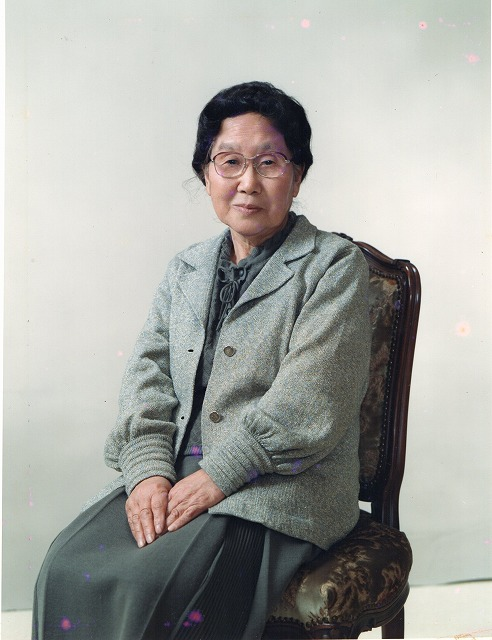
\includegraphics[height=9cm, angle=90, bb=0 0 640 640]{cat.jpg}
\begin{minipage}<y>[t]{6cm}
           福岡山下写真館
\end{minipage}
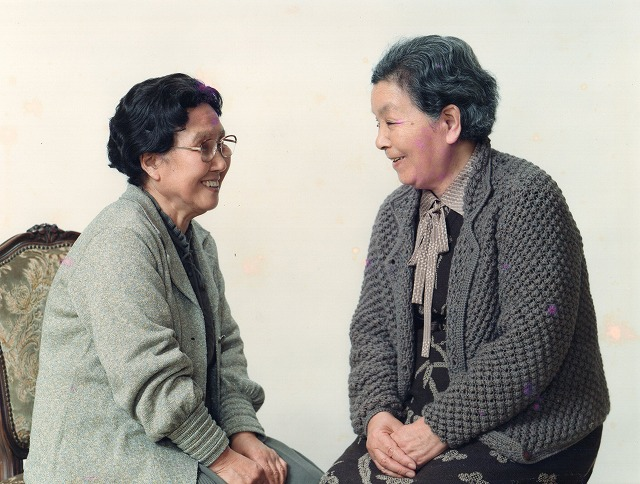
\includegraphics[height=9cm, angle=90, bb=0 0 640 640]{fumiko2.jpg}]\begin{minipage}<y>[t]{6cm}
           山下光子さんと
\end{minipage}




\end{document}

\end{document}
---------------------------------------------------------------------
\makeatletter
\newenvironment{shiika}
{\let\\\@normalcr\par
 \list{}{kanjiskip=0.25zw plus 0.01zw minus 0,01zw
  \xkanjiskip=\kanjiskip
 \utemsepz@ \topsep=\z@ \paesep=\z@
 \leftmergin=4zw \itemindeby=-2zw
\listparindentitemindeny \rightmargin=-zw }
 \iterekax}{\par\endlist}
\makeatother



==========================================================================
